\chapter{Experiments on real hardware}
In this chapter, the experiments conducted on the hardware system are discussed. The content is organized into four sections. An overview of the hardware setup for the double pendulum system is provided in the first section. The system identification of the hardware is delved into in the second section. The approach to addressing the sim-to-real gap challenge is detailed in the third section. The outcomes of the hardware experiments are presented in the final section.

\section{Hardware setup}
To be clear upfront, the hardware design and manufacturing were completed by previous researchers and coworkers at the Underactuated Lab of the German Research Center for Artificial Intelligence GmbH, Robotics Innovation Center branch. My role in this section is to understand the logic of all the involved subsystems and set up the test environment using existing components.

Mechanically, the double pendulum system is a straightforward 2-R linkage. The first revolute joint attaches to the base, while the second one connects the two links. Quasi-direct drive motors are mounted on each joint to provide torque, and a counterweight is positioned at the end of the second link.

The mechanical design of the double pendulum underwent two iterations. The initial design was characterized by rotational imbalances due to a slightly misaligned motor axis and homogeneous link sizes, leading to vibrations and potential failures. Significant improvements were made in the second iteration: the original aluminum-plastic links were replaced with a carbon fiber-foam composite, and a lightweight, triangular design with central cutouts was introduced. These changes not only rectified the weaknesses of the previous design but also resulted in a mechanical structure that was markedly more reliable and safer, with enhanced yield strength and reduced safety risks.

\begin{figure}[H]
    \centering
    \begin{subfigure}[b]{0.3\textwidth}
        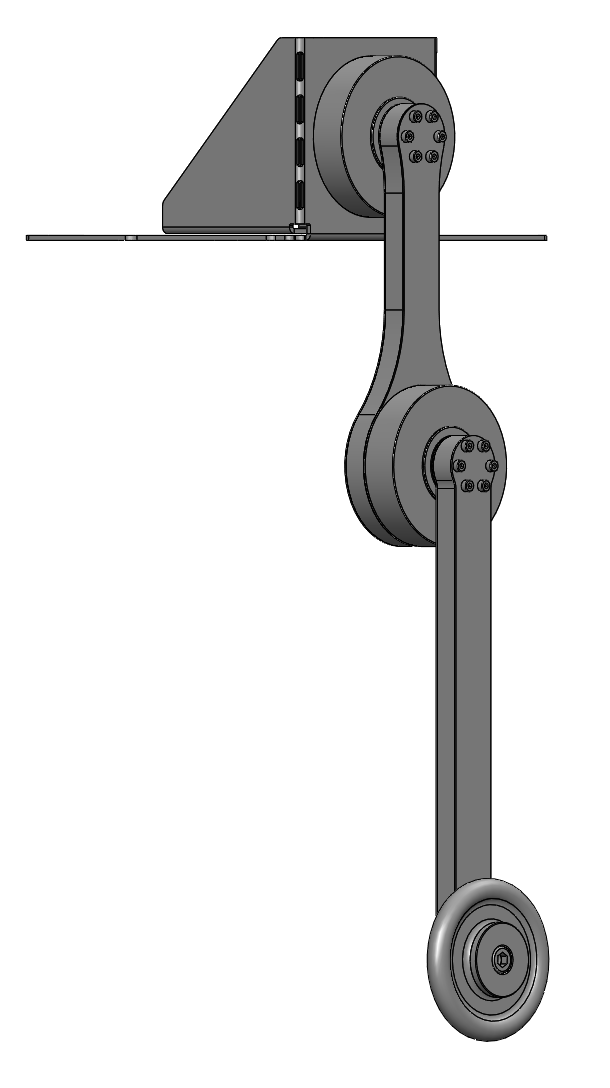
\includegraphics[width=\textwidth]{figures/hardware_setup/double_pendulum_it1_v1.png}
        \caption{Iteration 1 in isometric view}
        \label{fig:image1}
    \end{subfigure}
    \hfill
    \begin{subfigure}[b]{0.3\textwidth}
        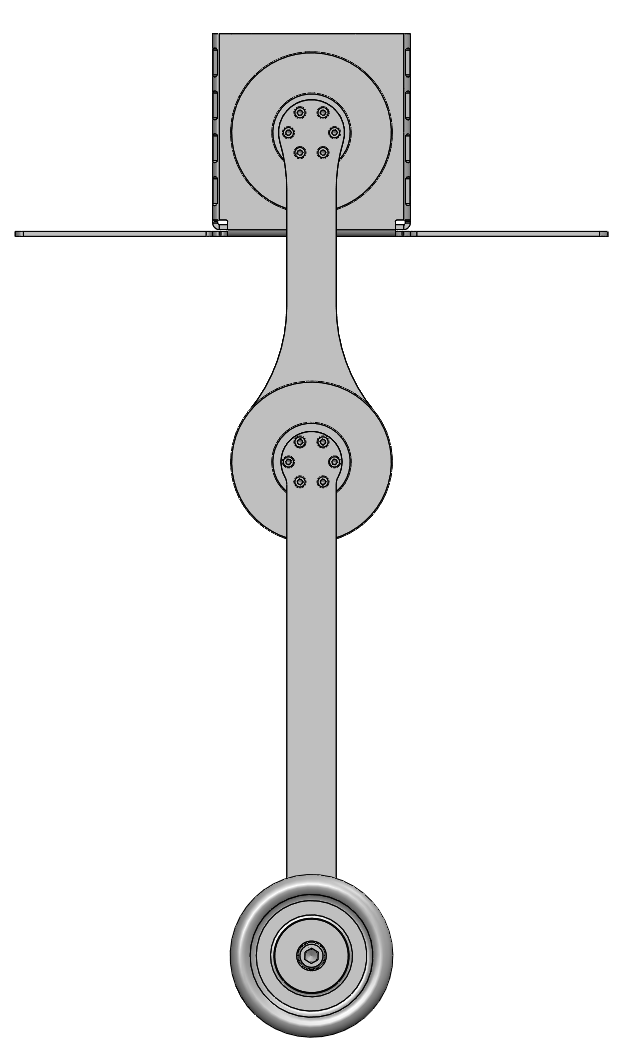
\includegraphics[width=\textwidth]{figures/hardware_setup/double_pendulum_it1_v2.png}
        \caption{Iteration 1 in front view}
        \label{fig:image2}
    \end{subfigure}

    \vspace{1em} % or use \bigskip or \medskip depending on the space you want

    \begin{subfigure}[b]{0.3\textwidth}
        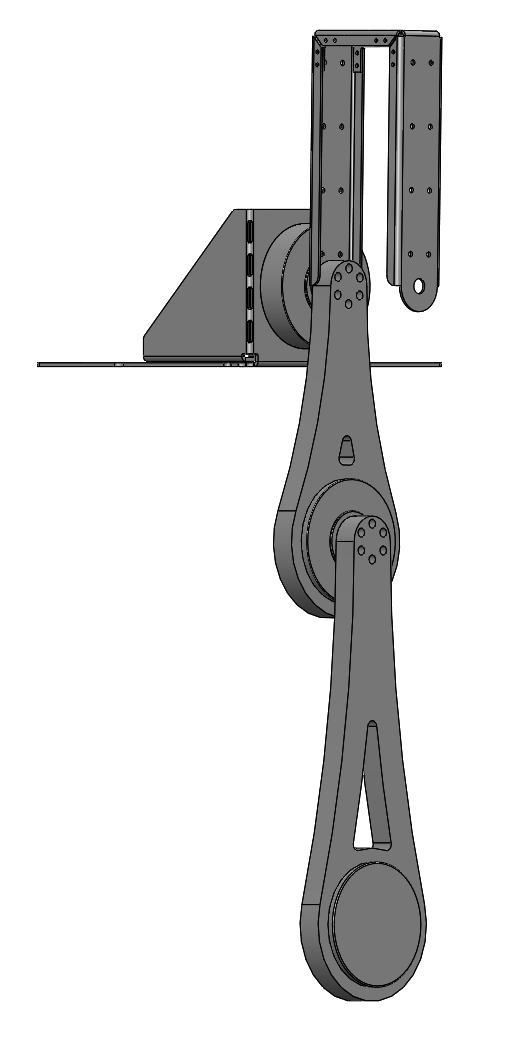
\includegraphics[width=\textwidth]{figures/hardware_setup/double_pendulum_it2_v1.png}
        \caption{Iteration 2 in isometric view}
        \label{fig:image3}
    \end{subfigure}
    \hfill
    \begin{subfigure}[b]{0.3\textwidth}
        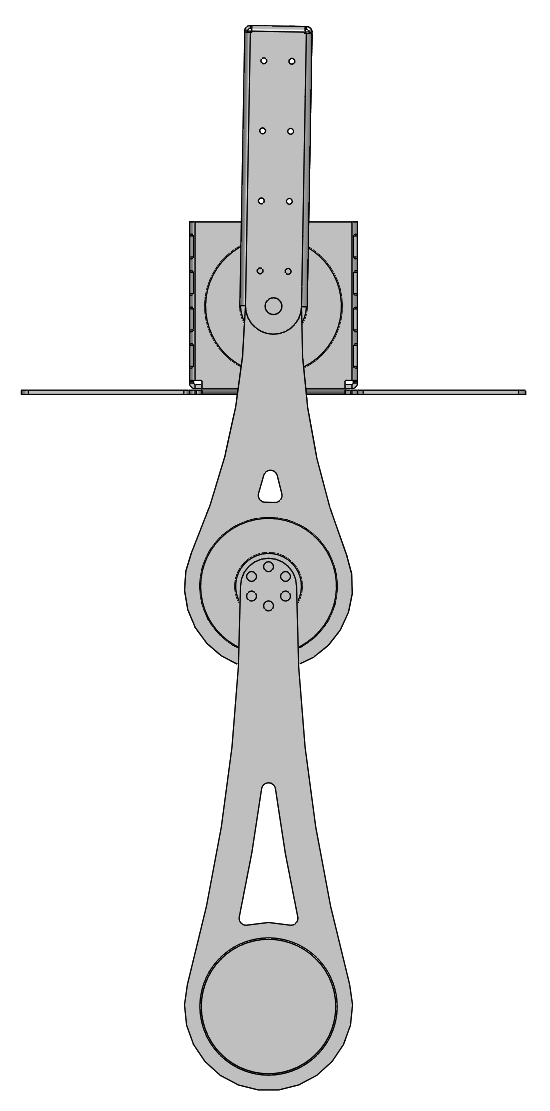
\includegraphics[width=\textwidth]{figures/hardware_setup/double_pendulum_it2_v2.png}
        \caption{Iteration 2 in front view}
        \label{fig:image4}
    \end{subfigure}
    \caption{Double pendulum mechanical system iteration 1 and iteration 2}
    \label{fig:four_images}
\end{figure}

For actuation selection, quasi-direct drive (QDD) motors were chosen. QDDs are popular choices for actuation in robotics, commonly utilized in applications that demand both high torque and precise control, such as robotic arms or exoskeletons. They represent a compromise between direct drive systems, which connect the load directly to the motor without any gear reduction, and traditional geared systems, which use gears to increase torque at the cost of speed and may introduce backlash. The advantages of employing QDDs are apparent: they offer high precision and allow for precise control. Furthermore, the low gear ratio simplifies joint dynamics, which can typically be neglected when modeling the overall system dynamics. The drawbacks, however, are also evident. QDDs are costlier than average motors, and the low gear ratio limits the torque output.

\begin{figure}[H]
  \centering
  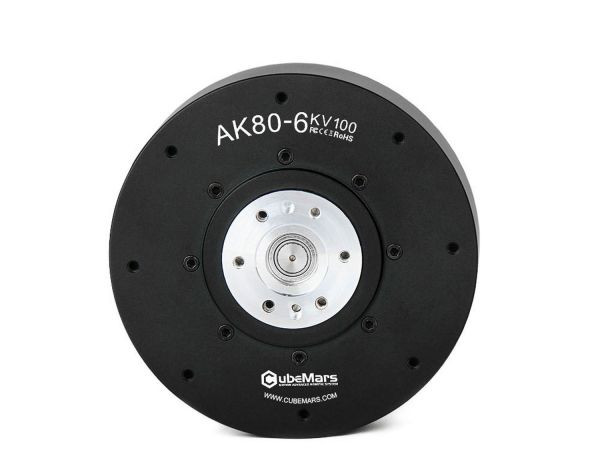
\includegraphics[width=0.5\textwidth]{figures/hardware_setup/motor.jpg}
  \caption{AK80-6 V100 motor\cite{cubemarsAK806}}
  \label{fig:AK80-6}
\end{figure}

The AK80-6 V100 motors from CubeMars were selected for their ease of mounting, which is facilitated from both the front and rear ends\cite{cubemarsAK806}. As shown in Figure \ref{fig:torque_speed_curve}, these motors are characterized by a peak torque of 12 Nm and a rated torque of 6 Nm during continuous operation, aligning with the project's set torque limit of 5 Nm. They are designed to operate on a 24V voltage with a gear ratio of 6:1. Additionally, their design incorporates compatibility with both serial and CAN bus systems, which simplifies the development process.

\begin{figure}[H]
  \centering
  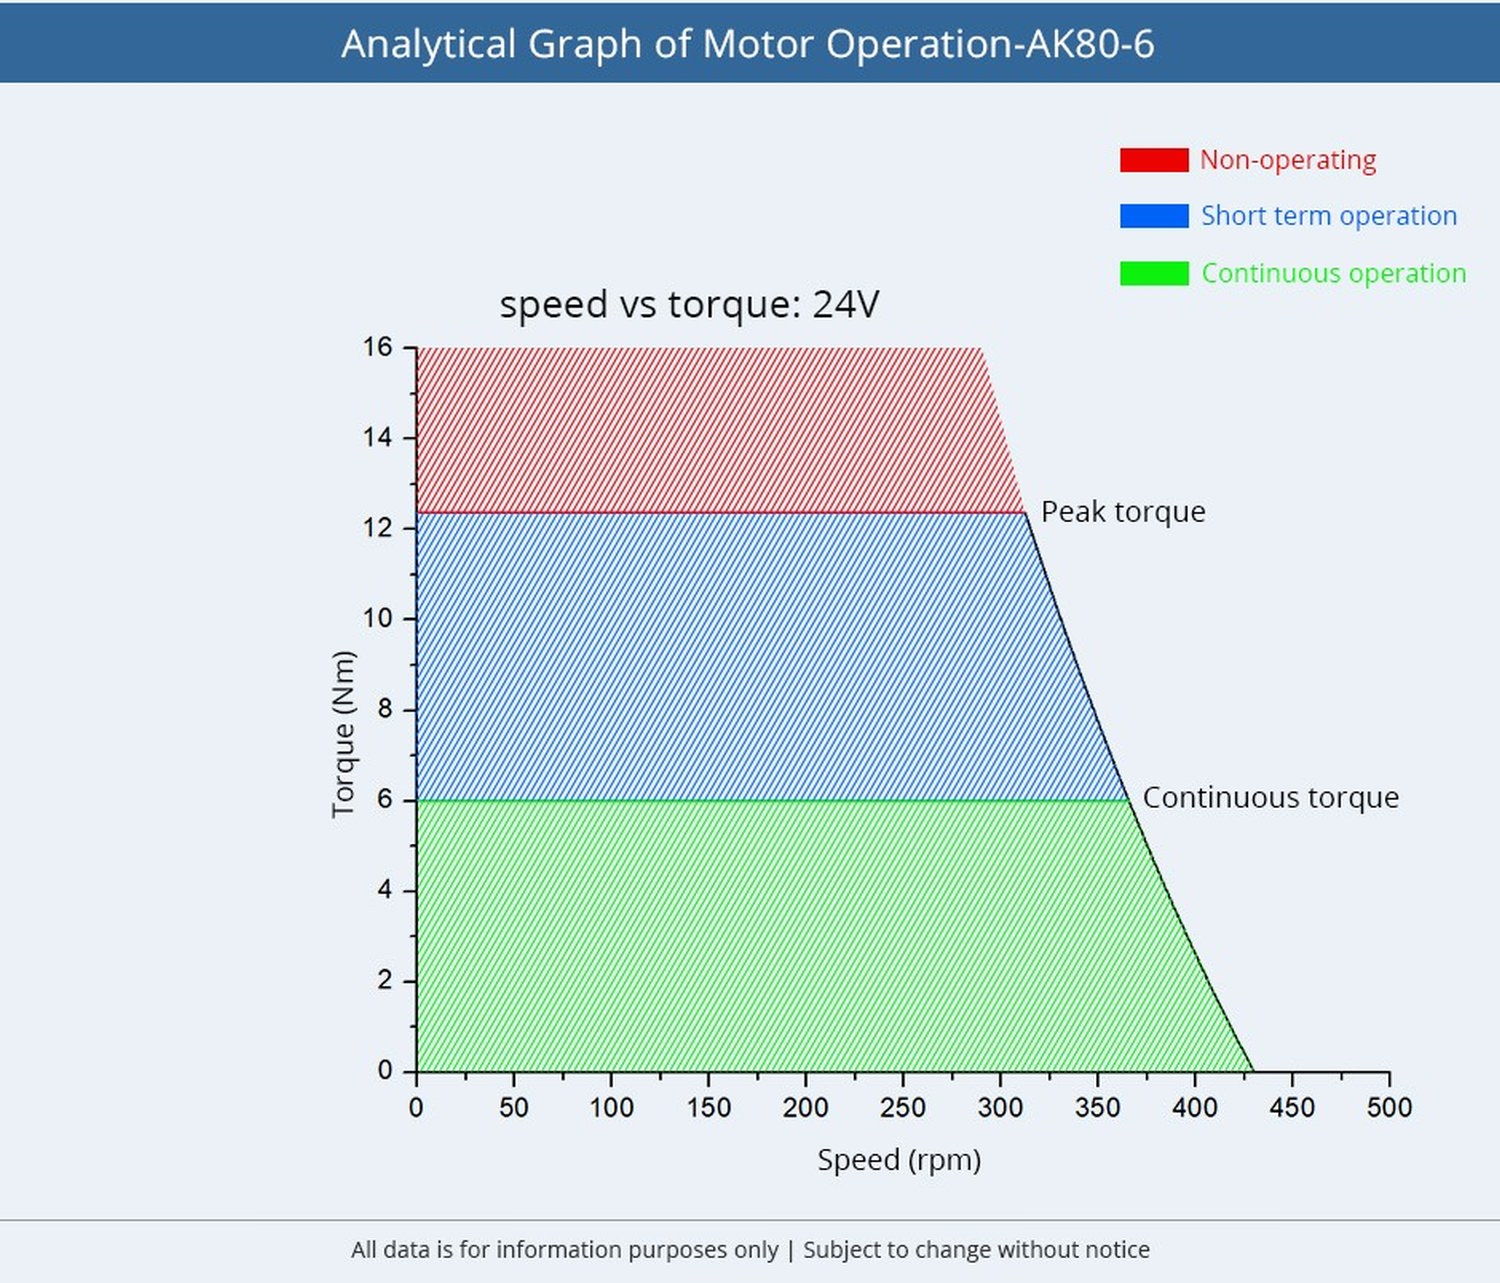
\includegraphics[width=0.80\textwidth]{figures/hardware_setup/torque_speed_curve.jpg}
  \caption{Torque speed curve of AK80-6 V100 motor\cite{cubemarsAK806}}
  \label{fig:torque_speed_curve}
\end{figure}

For communication, the Controller Area Network (CAN) bus was chosen due to its compatibility with the actuators. Known for its robustness, flexibility, and efficiency, the CAN bus is a communication protocol that has been widely utilized in various applications. The adoption of the CAN bus for control brings numerous advantages. It provides error checking and fault confinement capabilities and supports real-time operation, facilitating high control frequencies with a relatively simple wiring arrangement. 

In our application (Figure \ref{fig:can_connection_diagram}), the network comprises one master node (the PC) and two slave nodes (the motors). The control loop is constituted by a CAN-to-USB converter, a single CAN high cable, and a single CAN low cable, with termination resistors of \(120 \Omega\) at both the initial and terminal points of the network.

\begin{figure}[H]
  \centering
  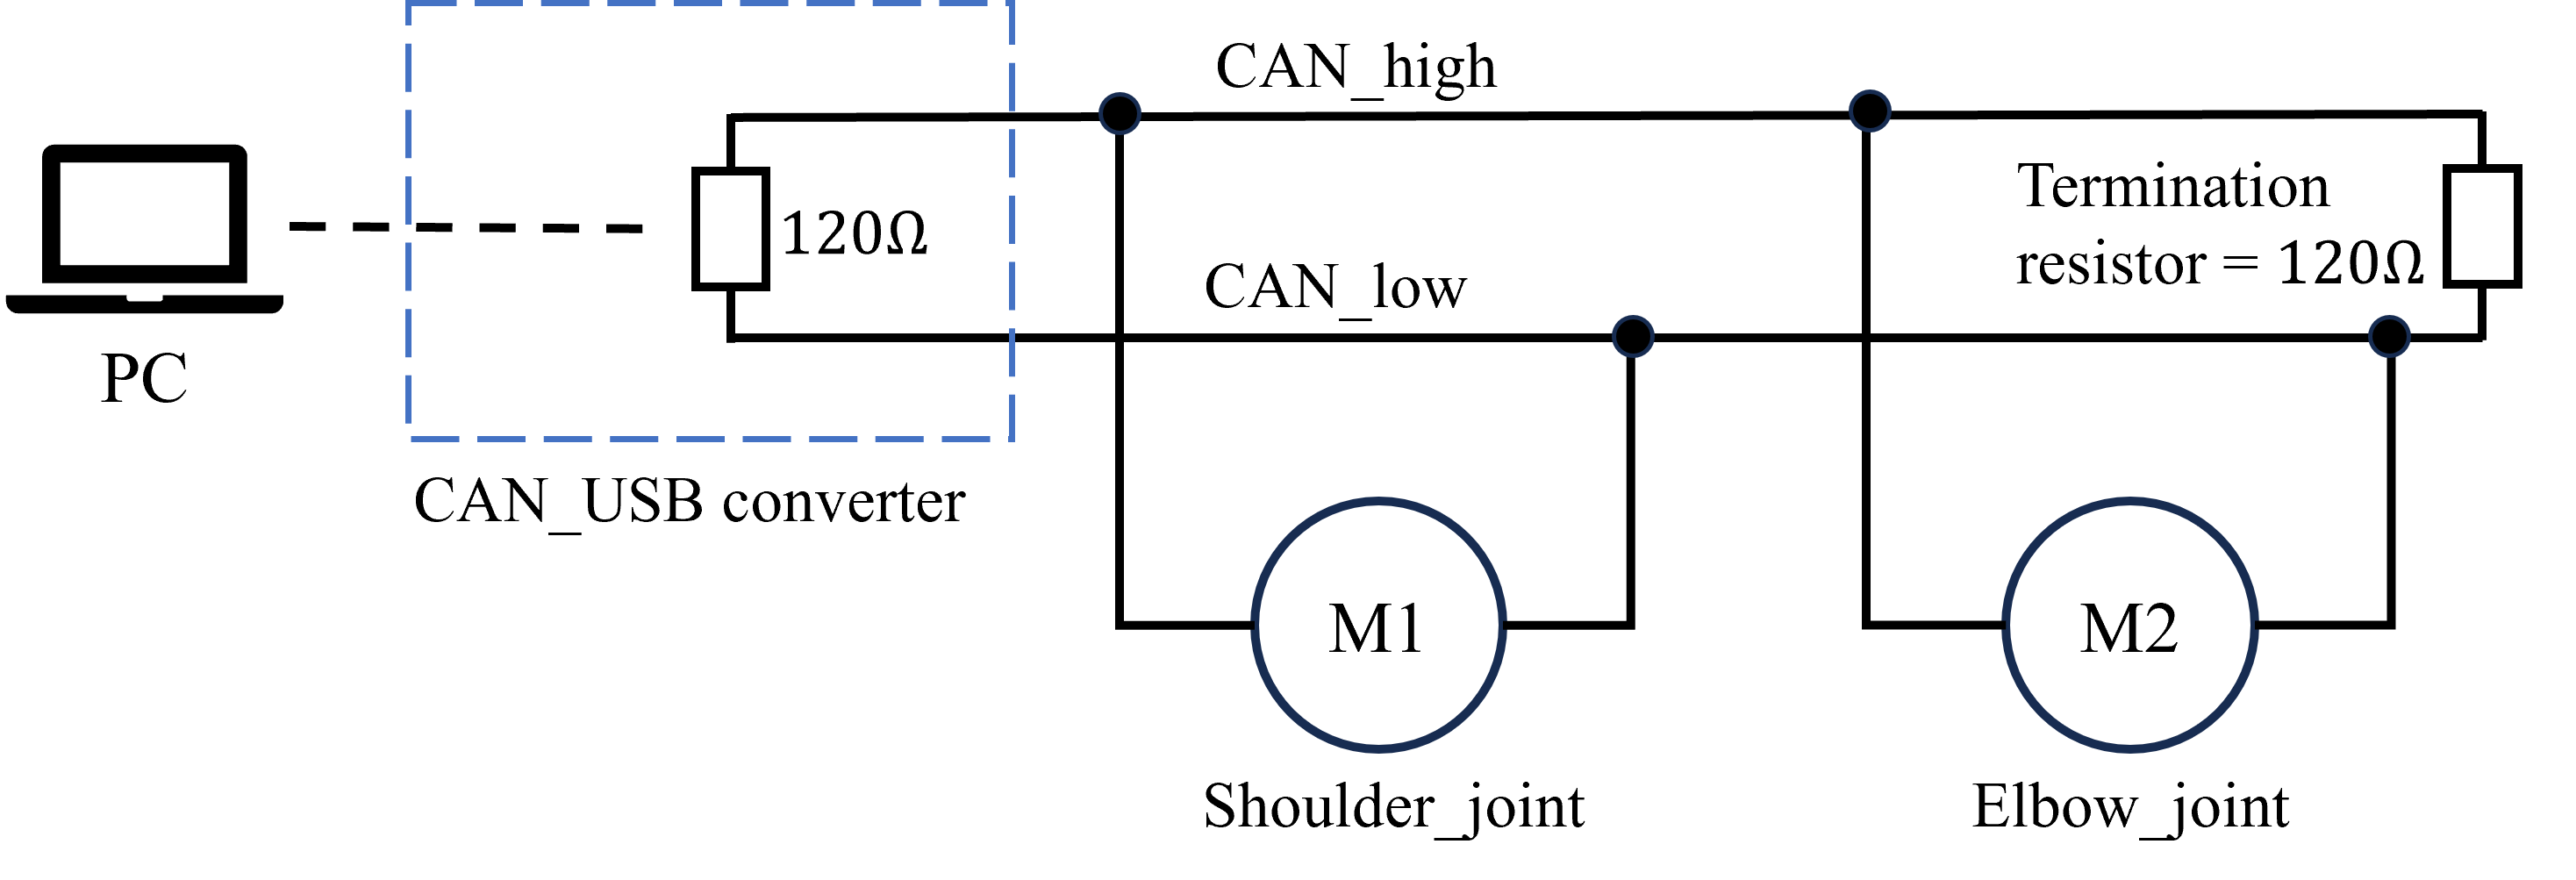
\includegraphics[width=0.9\textwidth]{figures/hardware_setup/can_connection.png}
  \caption{CAN connection diagram}
  \label{fig:can_connection_diagram}
\end{figure}

To achieve a higher control frequency of approximately 500 Hz, the CAN-USB/2 product from ESD GmbH Hannover~\cite{esdCANUSB2} was selected. This specialized interface exploits the USB 2.0 standard, which allows for a data rate of 480 Mbit/s, and features CAN capability at 1 Mbit/s as per ISO 11898-2. Furthermore, compatibility with the SocketCAN interface, which is incorporated into the Linux Kernel 2.6, is supported, thereby facilitating its use within a Linux development environment.

\begin{figure}[H]
    \centering
    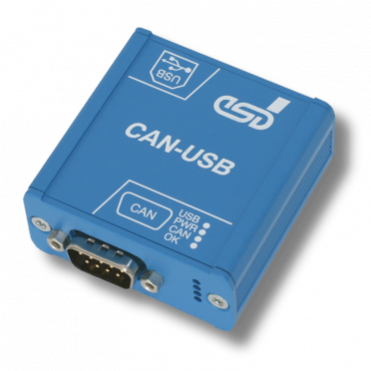
\includegraphics[width=0.3\linewidth]{figures/hardware_setup/can_blue_box.png}
    \caption{High speed CAN to USB interface\cite{esdCANUSB2}}
    \label{fig:can_blue_box}
\end{figure}

Following accidents encountered during testing with the initial mechanical systems, several safety protocols have been instituted to safeguard human lives and equipment. Four principal measures are now in place.

\textbf{Emergency stop:}

An emergency stop has been interfaced directly with the 24V power supply. In the event that the double pendulum's behavior deviates from the expected parameters during tests, the power can be disconnected manually with immediate effect. Subsequently, the mechanical system's energy will dissipate swiftly, causing an automatic reversion to its initial state.

\textbf{Capacitor:}

In instances where the emergency stop is activated while the system operates at high velocities, the motors at the revolute joints serve as generators, converting the mechanical energy into electrical energy. This conversion process results in a current that is channeled back into the circuit, which, under extreme conditions, has the potential to overload the power supply. To mitigate this, a capacitor has been incorporated into the power supply circuitry to capture any excessive electrical energy that may arise from the abrupt cessation of the system's movement.

\begin{figure}[H]
    \centering
    \includegraphics[width=0.4\textwidth]{figures/hardware_setup/capacitor.jpg}
    \caption{Capacitor}
    \label{fig:capacitor}
\end{figure}

\textbf{Speed and position limit:}

At the software level, speed and position limits have been defined. Due to the potential for vibrations and rotational imbalances that may occur at high speeds, which could lead to structural disassembly, a maximum speed of \(20\) rad/s has been instituted. Should the speed surpass this threshold, an automatic system halt will be initiated, analogous to the actuation of the emergency stop mechanism. Position limits have been established at \(2\pi\) for both joints. Excessive rotations risk the entanglement of CAN and power cables, which could result in interference and possible cable damage. A schematic of the entire wiring system is illustrated in the Figure \ref{fig:wiring diagram}:

\textbf{Physical enclosure:}

A custom-designed enclosure(see Figure \ref{fig:overview_experiment_setup}) has been fabricated to serve as a safeguard against unanticipated system failures. Constructed from aluminum profiles and reinforced with thick acrylic boards, the enclosure comprehensively surrounds the double pendulum apparatus, significantly mitigating the potential for accidents.

These safety measures have been crucial in reducing the risks associated with testing and operational procedures.

\begin{figure}[H]
    \centering
    \includegraphics[width=0.9\textwidth]{figures/hardware_setup/enclosure.jpg}
    \caption{Physical enclosure for protection}
    \label{fig:overview_experiment_setup}
\end{figure}

\begin{figure}[H]
    \centering
    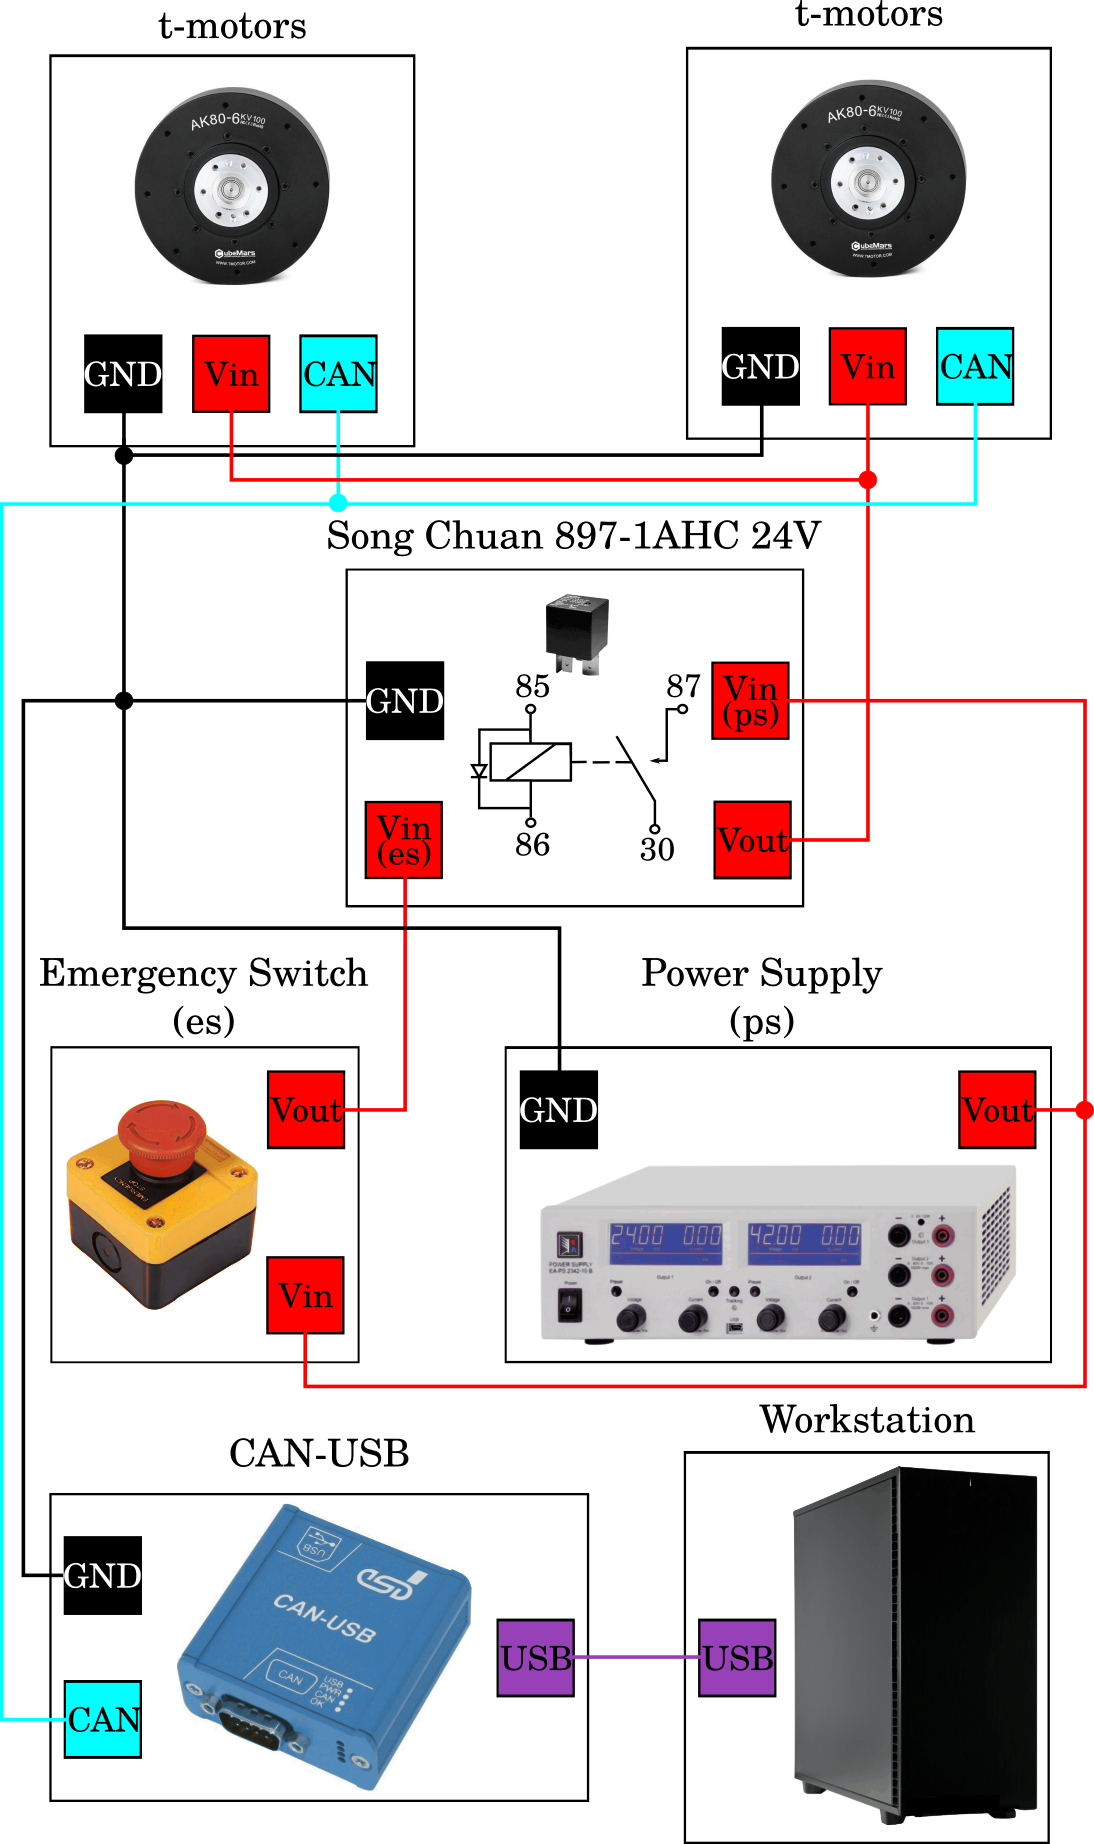
\includegraphics[width=0.7\linewidth]{figures/hardware_setup/wiring-diagram.png}
    \caption{Wiring diagram\cite{2023_ram_wiebe_double_pendulum}}
    \label{fig:wiring diagram}
\end{figure}

\section{System identification}
Before implementing control strategies on a real system, it is crucial to ensure that the dynamics of the real system match those anticipated in theory. To achieve this, identifying the values used in the equation of motion is essential, and the system identification method is employed.

System identification is the process of deriving mathematical models of dynamic systems from observed input-output data. This method is widely used in control theory to analyze and predict the behavior of real-world systems. The common procedure of system identification includes model structure selection, data collection, and parameter estimation.

\textbf{Model Structure Selection:}

As described in Section 2.1.2, the equation of motion for the target system is derived using the Lagrangian method, as expressed in Equation \ref{eq:EoM}. Fifteen parameters are required to fully describe the system dynamics, including masses $(m_1, m_2)$, lengths $(l_1, l_2)$, centers of masses $(r_1, r_2)$, inertias $(I_1, I_2)$ for the two links, and six actuator parameters, namely motor inertia $I_r$, gear ratio $g_r$, Coulomb friction $(c_{f1}, c_{f2})$, and viscous friction $(b_1, b_2)$ for the two joints, and gravity $g$.

While the naturally provided parameters $g$ and $g_r$ are held constant, the easily measurable parameters $l_1$ and $l_2$ are measured by hand and recorded in Table \ref{tab:different_designs}. The remaining 11 system parameters need to be determined. We define the following terms as independent variables, which are to be estimated during the system identification experiment:

\[m_1 r_1, m_2 r_2, m_1, m_2, I_1, I_2, I_r, b_1, b_2, c_{f1}, c_{f2}\]

\textbf{Data Collection:}

System identification experiments are conducted by running excitation trajectories on the real hardware. The excitation trajectories include inputs of $[t, q, \dot{q}, \ddot{q}]^T$, where $t$ is the timestamp, $q = [p_1, p_2]^T$ represents position, $\dot{q} = [v_1, v_2]^T$ represents velocity, and $\ddot{q} = [a_1, a_2]^T$ represents acceleration. Data tuples in the form $(q, \dot{q}, \ddot{q}, u)$ can be collected. One of the excitation trajectories are shown in Figure \ref{fig:excitation_traj}.

\begin{figure}[H]
    \centering
    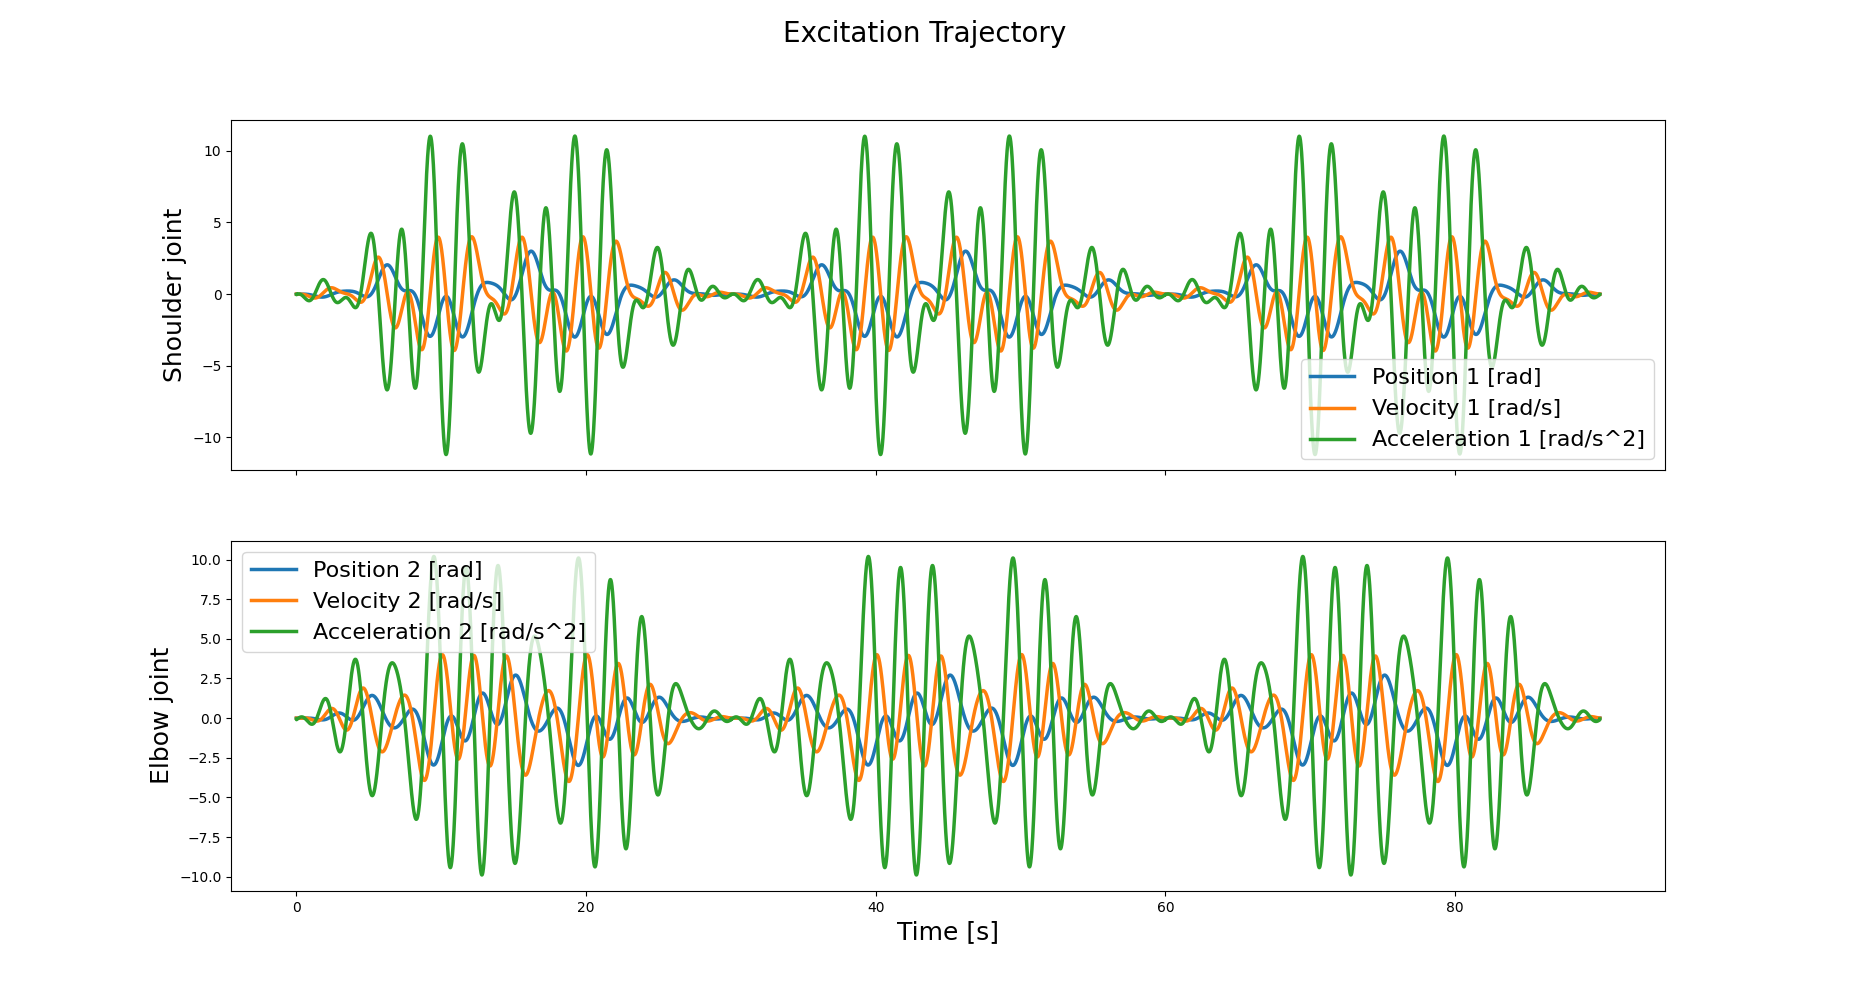
\includegraphics[width=1.1\linewidth]{figures/hardware_setup/excitation_traj.png}
    \caption{Excitation trajectory}
    \label{fig:excitation_traj}
\end{figure}

\textbf{Parameter Estimation:}

To determine the most accurate system parameters, a least squares optimization can be performed on the recorded data. The objective of the least squares optimization is to find the values of model parameters that minimize the sum of squared differences between the observed output data and the model's predictions. The objective function can be expressed as:

\begin{equation}
J(\theta) = \sum (y_{\text{observed}} - y_{\text{predicted}}(\theta))^2
\end{equation}

Where:
\begin{itemize}
\item $J(\theta)$ is the cost function to be minimized.
\item $\theta$ represents the vector of model parameters to be estimated.
\item $y_{\text{observed}}$ is the vector of observed output data.
\item $y_{\text{predicted}}(\theta)$ is the vector of model predictions based on the current parameter values $\theta$.
\end{itemize}

The optimization uses the CMA-ES (Covariance Matrix Adaptation Evolution Strategy) algorithm\cite{hansen2001completely}, and the identified model parameters are shown in Table \ref{tab:parameters}. These parameters are based on design C ($l_1 = 0.2m$, $l_2 = 0.3m$), which is used in real-world tests.

\begin{table}[H]
\centering
\begin{tabular}{|c|c|}
\hline
\textbf{Parameter} & \textbf{Value} \\
\hline
$I_1$ & 0.031887199591513114 \\
$I_2$ & 0.05086984812807257 \\
$I_r$ & 6.287203962819607e-05 \\
$b_1$ & 0.001 \\
$b_2$ & 0.001 \\
$c_{f1}$ & 0.16 \\
$c_{f2}$ & 0.12 \\
$g$ & 9.81 \\
$g_r$ & 6.0 \\
$l_1$ & 0.2 \\
$l_2$ & 0.3 \\
$m_1$ & 0.5234602302310271 \\
$m_2$ & 0.6255677234174437 \\
$r_1$ & 0.2 \\
$r_2$ & 0.25569305436052964 \\
\hline
\end{tabular}
\caption{Parameter values from system identification}
\label{tab:parameters}
\end{table}


\section{Sim-to-Real transfer}
Transferring working models from simulation to real systems to produce similar performance has always been a challenge in controller design. This challenge is even more pronounced in model-free reinforcement learning for two main reasons.

Firstly, model-free reinforcement learning relies solely on interaction with the environment to gain experience and select actions. While a simulation environment is merely a simplification of the real-world scenario, the agent in simulation might not capture all the factors, such as friction, sensor noise, or real-world dynamics, accurately. Therefore, a control policy optimized for a simplified model might not perform as expected in the more intricate real world.

Secondly, many simulations operate in discrete time and space, whereas the real world functions continuously. In our implementation, the control frequency presents a significant challenge. We use a control frequency of 100 Hz in simulation; however, it does not suffice in the real system. To enhance performance, we increased the control frequency to 400 Hz when experimenting on the real system, and this adjustment yielded positive results.

\subsection{Validation with noisy simulation environment}
In addressing the challenge of sim-to-real transfer, multiple agents were trained using the Soft Actor-Critic (SAC) algorithm under similar setups in an ideal environment. These agents were then subjected to validation within a noisy environment, which is an ideal environment incorporated with real-world features. Only those agents demonstrating robustness to perturbations within this environment were advanced to real-world tests. Agents that did not withstand the noisy environment were deemed insufficiently robust and subsequently discarded.

In the course of real world experiments, four critical factors were identified that differ from ideal simulations: friction, measurement noise, latency, and torque responsiveness.

\textbf{Friction:}

Friction, identified as the predominant factor affecting performance, was not accounted for in the simulated training environment. To bridge this gap with real-world conditions, a friction compensation strategy was employed, starting with modeling the friction based on Coulomb’s law as detailed in Equation \ref{eq:friction_function}. 

Since frictional force counteracts the relative motion between contact surfaces, this compensation involved exerting additional torque in the same direction as the angular motion, providing the system with the necessary energy to overcome the effects of friction.

Despite the friction coefficients \(c_{f1}\) and \(c_{f2}\) being ascertained during the system identification phase, they were subsequently found to be imprecise during real system testing. To refine these coefficients, free-fall tests were conducted, which entailed releasing the double pendulum from a slight angular displacement and allowing it to descend under the force of gravity. Given the coupling influence of the two links, one joint was immobilized during the friction coefficient tuning of the other: the elbow joint remained static while estimating the shoulder joint's coefficient, and vice versa. Manual adjustments to the friction coefficients were made until the position output of the tested joint resulted in a sine wave without decay.

\textbf{Measurement noise:}

Measurement noise has been identified as the second most critical factor. The position displacement is measured with high accuracy using built-in encoders in the AK80-6 motors. However, the velocity measurement, which is derived as the first derivative of the position measurement, tends to introduce a relatively higher error. In the ideal environment, measurement error for both position and velocity is assumed to be non-existent. Nonetheless, this error is considerable in real-world applications.

To tackle this problem, the measurement error has been modeled as a normal distribution, with the mean representing the true velocity value and a manually adjustable standard deviation. The measurement noise vector is denoted by \(\epsilon = [\Delta p_1, \Delta p_2, \Delta v_1, \Delta v_2]^T\), and is assumed to follow a multivariate normal distribution:
\begin{equation}
\epsilon \sim \mathcal{N}(\boldsymbol{\mu}, \boldsymbol{\Sigma})
\end{equation}
where \(\boldsymbol{\mu}\) is the vector of means, and \(\boldsymbol{\Sigma}\) is the \(4 \times 4\) covariance matrix, representing the uncertainty spread of the noise across each dimension. The measurements for the four states are presumed to be independent, rendering \(\boldsymbol{\Sigma}\) a diagonal matrix. In practice, \(\mu = 0\) and \(\Sigma = \text{diag}(0,0,0.5,0.5)\), indicating an omission of measurement noise on positions and a focus on the velocity measurement noise.

\textbf{Latency:}

Latency has been identified as the third significant factor. Given that any communication system requires time to transmit and receive data, and programs also require time to execute, latency is an inevitable aspect. Such latency presents a substantial challenge to control systems, especially those based on reinforcement learning. Reinforcement learning operates on the principles of Markov Decision Processes (MDPs), which follow the Markov property. According to this property, the future state of a MDP process is determined solely by the current state and action, and not by the sequence of states that preceded it. However, latency compromises the Markov property by inducing state mismatches and fostering dependencies on historical data. During free-fall tests, the maximum latency observed was 0.015 seconds. Therefore, this value has been established as the standard latency.

\textbf{Torque responsiveness:}

The fourth factor to be considered is torque responsiveness. In real hardware tests, it was observed that motors struggle to match the torque output with rapidly alternating control signals, particularly when there are significant differences between consecutive time steps. To model this phenomenon in noisy simulation, a discount coefficient \( c_{tr} \) is applied to the change in control signals. The actual applied torque \(u_{\text{real}}\) is the sum of the previous torque \(u_{\text{previous}}\) plus the discounted change in torque \(u_{\text{current}} - u_{\text{previous}}\). The calculation is expressed as follows:

\begin{equation}
 u_{\text{real}} = u_{\text{previous}} + c_{tr} \cdot (u_{\text{current}} - u_{\text{previous}})
\end{equation}

When \(c_{tr}\) equals zero, the torque that is exerted on the system precisely mirrors the controller's output. A lower \(c_{tr}\) value makes it more difficult to apply significant changes to the control signal. Conversely, a policy that functions effectively with a low \(c_{tr}\) value indicates better torque smoothness. This also acts as an intuitive measure of the policy's capacity to yield smooth torque outputs. In most cases, \(c_{tr}\) is set to 0.85; however, to test the controllers' boundaries, values below 0.7 are also examined.

\subsection{Noisy training based on domain randomization}
For agents that succeeded in ideal simulations yet failed in noisy simulations, domain randomization has been identified as one method to enhance robustness.

Domain randomization \cite{tobin2017domain}, a technique conceived to narrow the gap between simulation and reality, aims to enable a model to operate effectively in real-world conditions, without the need for labeled real-world training data.

Initially emerging from the computer vision domain, domain randomization involves training a model not within a single, static simulation but rather within a diverse and perturbed environment. This is achieved by incorporating random variations into the ideal simulation. Techniques commonly employed in vision-based systems include changing the colors and textures of objects, modifying the lighting conditions, adjusting object shapes and sizes, introducing random noise to sensor data, and perturbing physical properties like friction or mass.

In the application of domain randomization to robotic manipulation tasks, disturbances introduced in the noisy simulation were employed to construct a noisy training process. This process resembles the previous ideal training process, but the environments for both the trial and evaluation phases were substituted with noisy environments. The training was warm-started with pretrained agents that had demonstrated success in ideal simulations yet performed poorly in noisy simulations.

The results of domain randomization in noisy training proved to be highly variable. Some agents significantly improved after a mere 5e6 iterations of noisy training, while others remained unchanged or worsened, with some even regressing to the point of failure in ideal simulations where they had once succeeded.


\section{Results on real hardware}
In this section, the results from the real hardware phase are presented. The content is divided into three parts. The first part discusses the procedure for selecting agents suitable for real-world testing. The second part displays the successful outcomes from an agent trained for the pendubot setup. The range of results is restricted to the pendubot setup due to the introduction of speed and position limits, which have significantly narrowed the range of possible policies. The third part discusses an unsuccessful agent in the acrobot setup. It passed ideal and noisy validations but cannot be transferred to real-world tests due to a violation of the \(2\pi\) position limit.

\begin{figure}[H]
    \centering
    \includegraphics[width=0.45\textwidth]{figures/double_pendulum_real_system.png}
    \caption{Double pendulum in real system}
    \label{fig:double_pendulum_real_system}
\end{figure}

\subsection{Agent selection procedure for real world tests}
An agent deemed suitable for real-system tests must undergo a process that includes training and validation in ideal environment, followed by validation in noisy environment. If the agent proves successful in noisy validation, it can proceed to further testing on the real system. If it does not succeed, we employ the domain randomization method in an attempt to enhance its performance. Should the retrained agent pass the noisy validation, it will then advance to real-system testing. Otherwise, it will be discarded.

\begin{figure}[H]
    \centering
    
\includegraphics[width=0.9\textwidth]{figures/hardware_result/agent_selection_procedure.png}% Second image
    \caption{Agent selection procedure for real hardware tests}
    \label{fig:agent_selection}
\end{figure}

\subsection{Pendubot results in real world}
All real hardware experiments are based on design C \( (l_1 = 0.2, l_2 = 0.3) \). For the pendubot setup, obtaining a working agent is relatively straightforward. Slight modifications were made to the training process for the ideal simulation phase by deactivating the scaling mechanism mentioned in Section 4.1 and adding a termination condition that ends the training episode if the shoulder or elbow joint exceeds \( 2\pi \), which means the agents are trained on unnormalized real physical state values with strict constraints on speed and velocity boundaries. Utilizing the parameters listed in Table~\ref{tab:training_parameters_real_world_pendubot}, the training process successfully yielded a working model in the ideal simulation within \( 2 \times 10^7 \) timesteps.

\begin{table}[H]
  \centering
  \begin{tabular}{p{2cm} | p{3cm} | p{3cm} | p{3cm}}
  Robot & Quadratic Reward  & Constant Reward & LQR\\
  \hline
  \multirow{5}{*}{Pendubot} & \(Q_1\) = 100 &  & \(Q_1\) = 0.97\\
  & \(Q_2\) = 100  & \(r_{line}=1e3\) & \(Q_2\) = 0.93\\
  & \(Q_3\) = 1.0  & \(r_{vel}=0.0\) & \(Q_3\) = 0.39\\
  & \(Q_4\) = 1.0  & \(r_{LQR}=1e5\)& \(Q_4\) = 0.26\\
  & \(R\) = 1e-2  & & \(R\) = 0.11\\
  \end{tabular}
 \caption{Hyper parameters used for training pendubot agents for real world tests}
 \label{tab:training_parameters_real_world_pendubot}
\end{table}

\begin{figure}[H]
    \centering
    \begin{subfigure}[b]{0.47\textwidth}
        \centering
        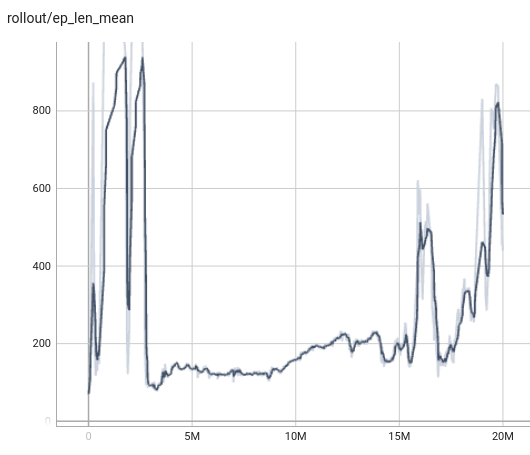
\includegraphics[width=\textwidth]{figures/hardware_result/train_without_limit_ep_length.png}
        \caption{Mean episode length}
        \label{fig:mean episode length}
    \end{subfigure}
    \hfill % add some horizontal spacing
    \begin{subfigure}[b]{0.47\textwidth}
        \centering
        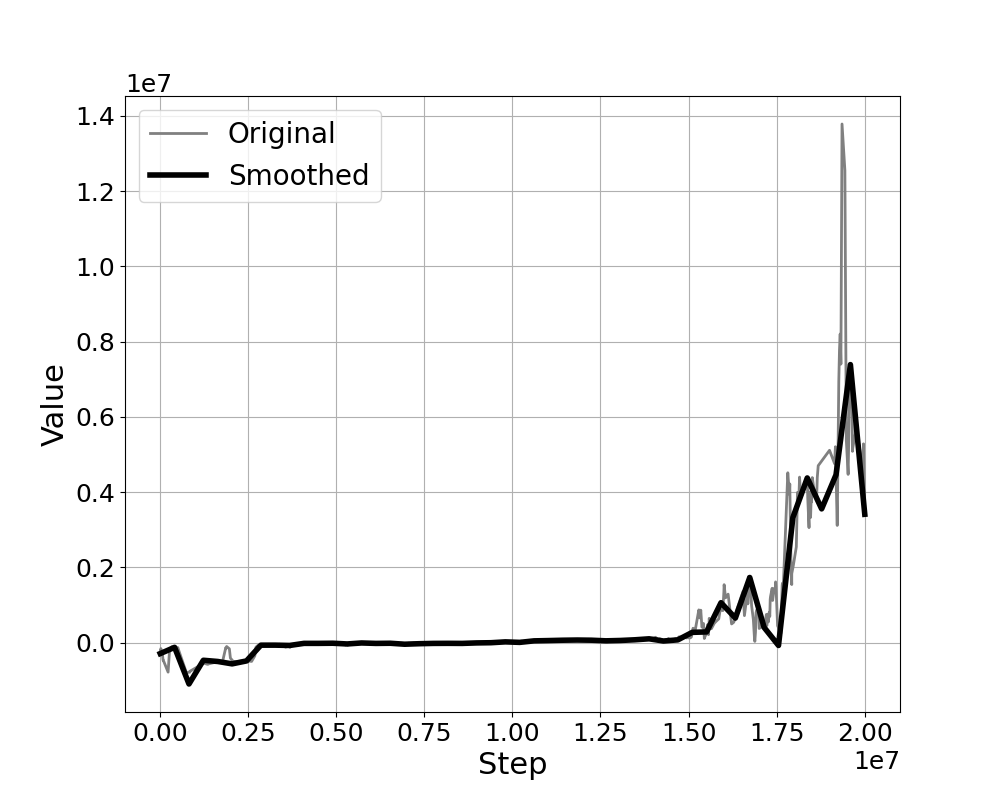
\includegraphics[width=\textwidth]{figures/hardware_result/train_without_limit_ep_reward.png}
        \caption{Mean episode reward}
        \label{fig:mean episode reward}
    \end{subfigure}
    \caption{Training curves of the working agent on pendubot}
    \label{fig:training_curves_for_real_world}
\end{figure}

Figure \ref{fig:training_curves_for_real_world} presents the training curve for the acquisition of an agent designated for real-world pendubot experiments, utilizing an ideal training process. As depicted in Figure \ref{fig:mean episode length}, the mean episode length initially approaches the maximum of 1000, but then it rapidly descends to below 200 after 3e6 training steps. This descent indicates that the agent consistently attempts to rotate beyond 360 degrees in pursuit of higher rewards. A sign of emergence from this performance valley is observed at 15e6 training steps, with a subsequent significant increase in episode length. Correspondingly, the mean episode reward, as illustrated in Figure \ref{fig:mean episode reward}, also shows a gradual increase before 15e6 time steps, followed by a rapid ascent thereafter.

The agent is put to the test in an ideal environment for validation. The results are 100\% successful, as shown in Figure \ref{fig:pendubot_ideal_working}. The switching time between the SAC controller and the LQR controller occurs in less than 1 second. After taking over, the LQR controller is able to maintain balance around the goal state until the end of the experiment.

\begin{figure}[H]
    \centering
    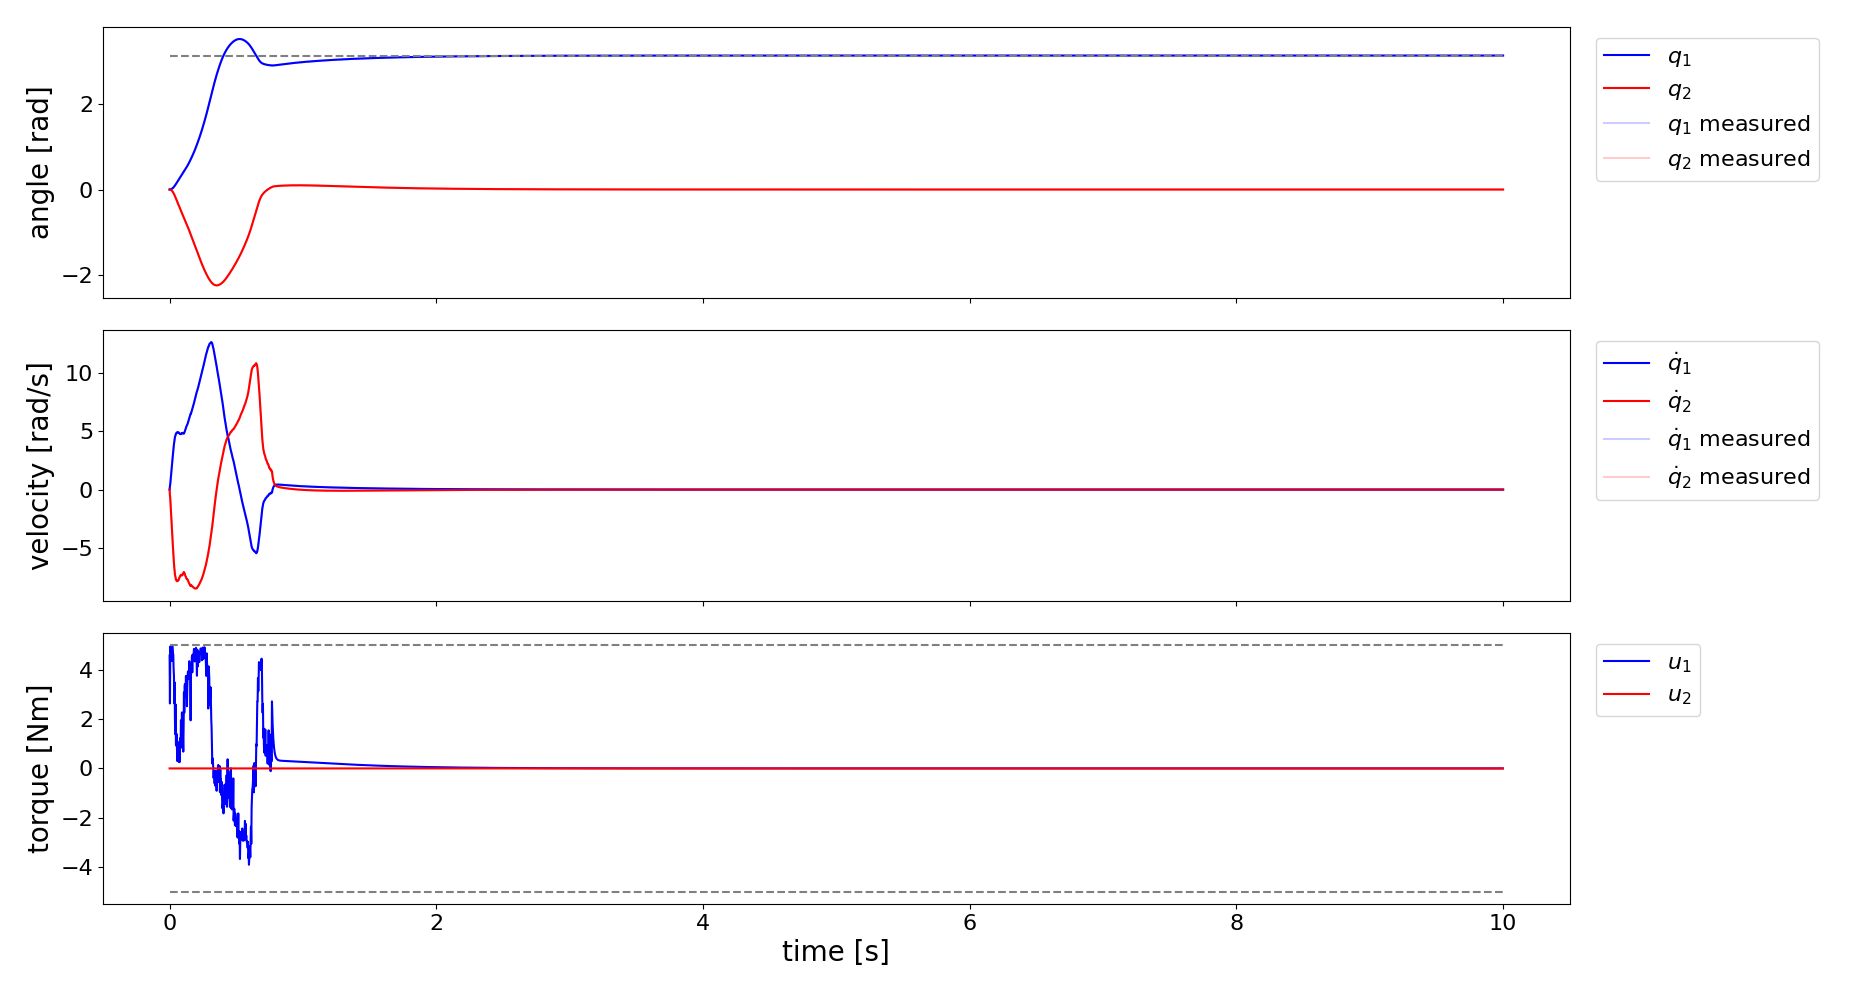
\includegraphics[width=0.95\linewidth]{figures/hardware_result/pendubot_ideal_validation_designC.1.png}
    \caption{Pendubot result in the ideal environment}
    \label{fig:pendubot_ideal_working}
\end{figure}

\begin{figure}[H]
    \centering
    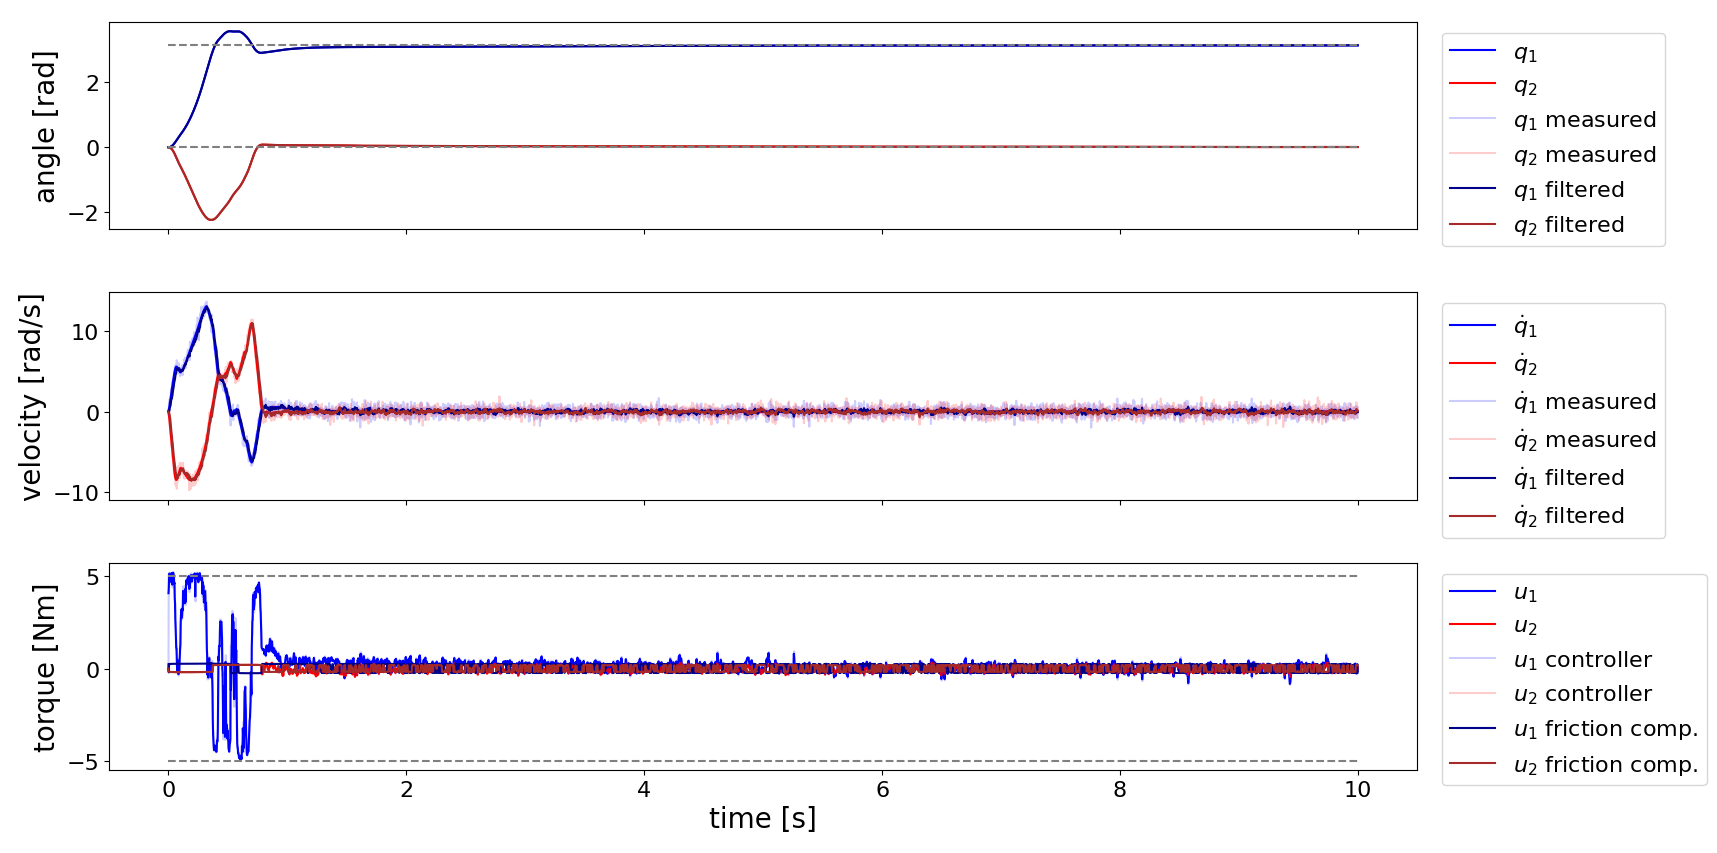
\includegraphics[width=1.0\linewidth]{figures/hardware_result/pendubot_noisy_simulation_designC.1.png}
    \caption{Pendubot result in the noisy environment}
    \label{fig:pendubot_noisy_working}
\end{figure}

Subsequently, the agent was subjected to noisy validation. In a noisy simulation, the pretrained agent was found to succeed at rate of 40\%, as demonstrated in Figure \ref{fig:pendubot_noisy_working}. In successful trials, the transition time between the SAC controller and the LQR controller occurred around 1 second. The LQR controller was still very effective in maintaining the system's stability. In unsuccessful trials, two scenarios occurred. Most often, the transition did not occur, and the system, remaining under the influence of the SAC controller, was inadequate for maintaining stability. In a few cases, although the transition did occur, the LQR controller failed to maintain the system's relative stable state around the upright position, resulting in experimental failure.

Though the noisy validation only have 40\% success rate, we consider the above shown agent ready for a real-world test, so we deploy it onto the test bench for the real world evaluation. A control frequency of 400Hz was utilized. The agent's average success rate in the real system was 40\%, aligning with the success rate observed during noisy validation. A depiction of one such successful outcome is presented in Figure \ref{fig:pendubot_real_working}. 

\begin{figure}[H]
    \centering
    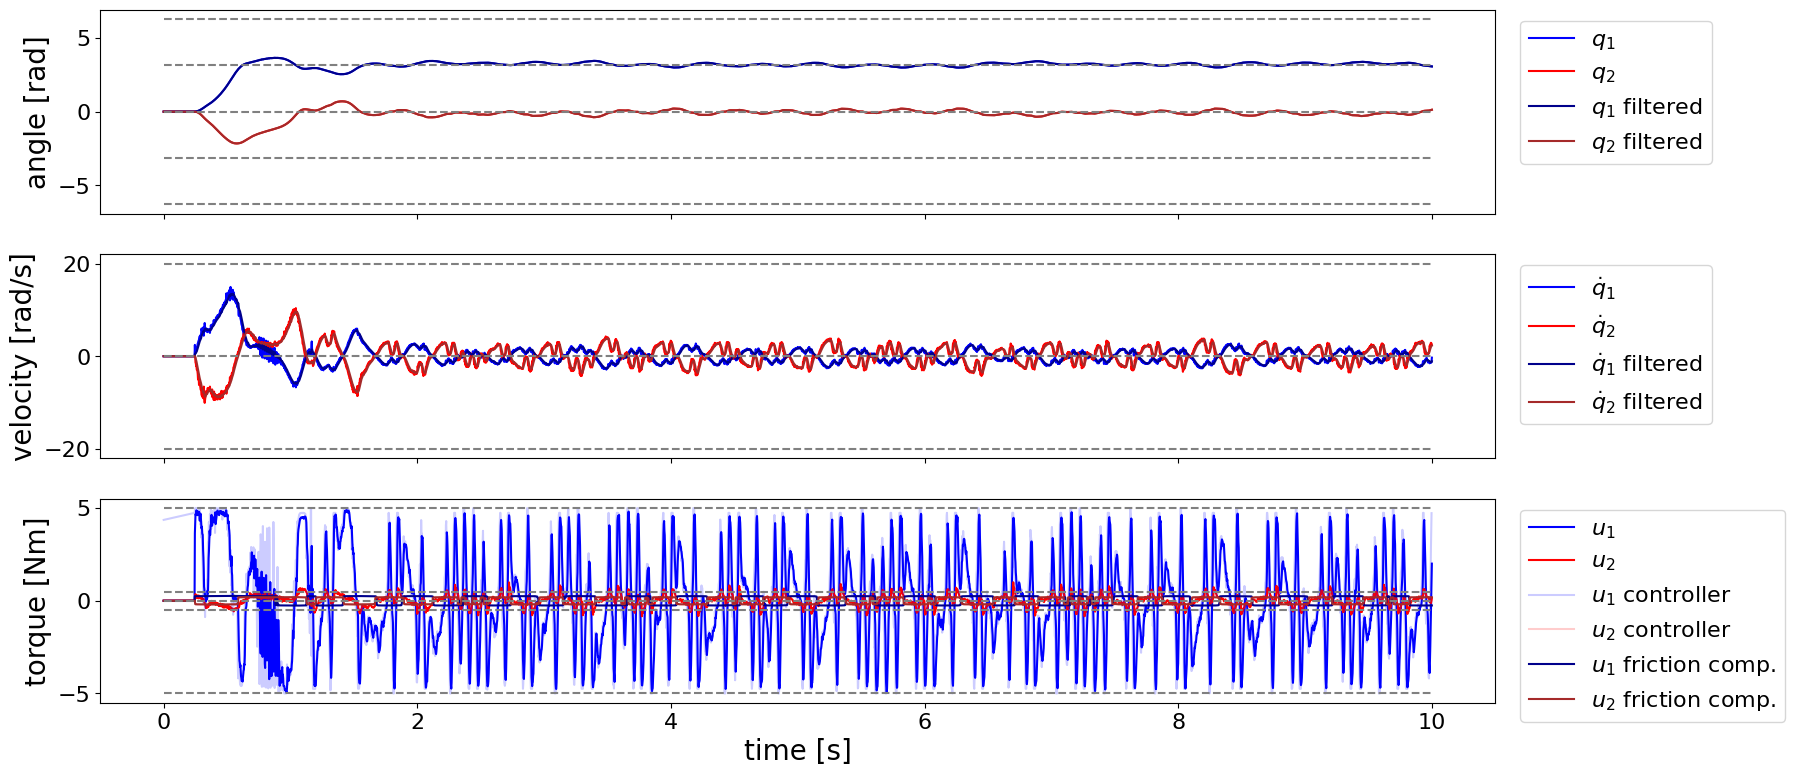
\includegraphics[width=1.0\linewidth]{figures/hardware_result/pendubot_real_system_working.png}
    \caption{Result of a successful pendubot experiment on real system}
    \label{fig:pendubot_real_working}
\end{figure}

The transition to the LQR controller occurred smoothly at approximately one second. Upon assuming control, the LQR controller succeeded in sustaining the system's upright position, albeit with vibrations, until the completion of the experiment. Contrary to the results in both noisy and ideal simulations, the torque applied by the LQR controller was noticeably less smooth, resulting in greater amplitude of position and velocity vibrations. Given that the feature of self-stabilization had been evident during the ideal validation phase, an attempt was made to omit the LQR controller, allowing the agent to execute the swing-up and stabilize independently; however, this approach proved unsuccessful.

In unsuccessful trials, similar problems that occurred during noisy validation recurred. The system either failed to switch from the SAC controller to the LQR controller, or the LQR controller was unable to maintain stability. The latter scenario is more likely to occur in real-world tests than in noisy validation.


\subsection{Acrobot results in real world}
Training for the acrobot setup has encountered numerous challenges, which can be summarized into the following aspects:

\textbf{Violation of Speed and Position Limit:}

The introduction of new rules, with a speed limit set at 20 rad/s and a position limit set at \(2\pi\), has made it more challenging to train a functional agent in the acrobot setup. Attempts have been made to train agents using unscaled real physical state values with a termination condition aimed at keeping the agent within the position limit; however, this approach did not perform as well as it did with the pendubot setup. Despite the application of 5e7 timesteps (which takes approximately 5 hours), neither the mean episode length nor the mean episode reward exhibited growth. A return to the method of training based on scaled state values without termination conditions eventually yielded a working model in ideal validation, although the \(2\pi\) position limit was violated.

\textbf{Inconsistency in Training:}

The training of acrobot agents has proven to be highly unstable. Despite the use of consistent and carefully tuned hyperparameters, training success has varied. There are instances when significant growth in mean episode reward suggests that training is progressing correctly, yet the resulting agent may perform inconsistently in ideal simulations.

\textbf{Long Training Hours:}

When compared to pendubot training, exploration in the acrobot setup often requires more time. While pendubot training typically produces a functional agent within 2e7 timesteps, acrobot training may take between 3e7 to 4e7 timesteps, with no guarantee that the resulting agent will pass an ideal validation. Such iterations, taking 3-4 hours each, are considerably time-consuming.

The most favorable outcome in the acrobot setup has been an agent that functions effectively in both ideal and noisy validations. It was trained using parameters detailed in Table \ref{tab:training_parameters_real_world_acrobot}, with an active scaling mechanism and in the absence of termination conditions, indicating that the agent was trained using normalized state values.

\begin{table}[H]
  \centering
  \begin{tabular}{p{2cm} | p{3cm} | p{3cm} | p{3cm}}
  Robot & Quadratic Reward  & Constant Reward & LQR\\
  \hline
  \multirow{5}{*}{Pendubot} & \(Q_1\) = 100 &  & \(Q_1\) = 1.92\\
  & \(Q_2\) = 90  & \(r_{line}=1e3\) & \(Q_2\) = 1.92\\
  & \(Q_3\) = 1.0  & \(r_{vel}=1e4\) & \(Q_3\) = 0.3\\
  & \(Q_4\) = 1.0  & \(r_{LQR}=1e5\)& \(Q_4\) = 0.3\\
  & \(R\) = 1e-2  & & \(R\) = 0.82\\
  \end{tabular}
 \caption{Hyper parameters used for training acrobot agents for real world tests}
 \label{tab:training_parameters_real_world_acrobot}
\end{table}

As shown in Figure \ref{fig:acrobot_training_curve}, the reward for this agent experienced a smooth increase up to 2.5e7 timesteps and then a rapid ascent in the final 5 million timesteps. Because a termination condition was not implemented, the episode length remained consistently at 1000. This outcome was anticipated and led to  a working agent in an ideal environment.

\begin{figure}[H]
    \centering
    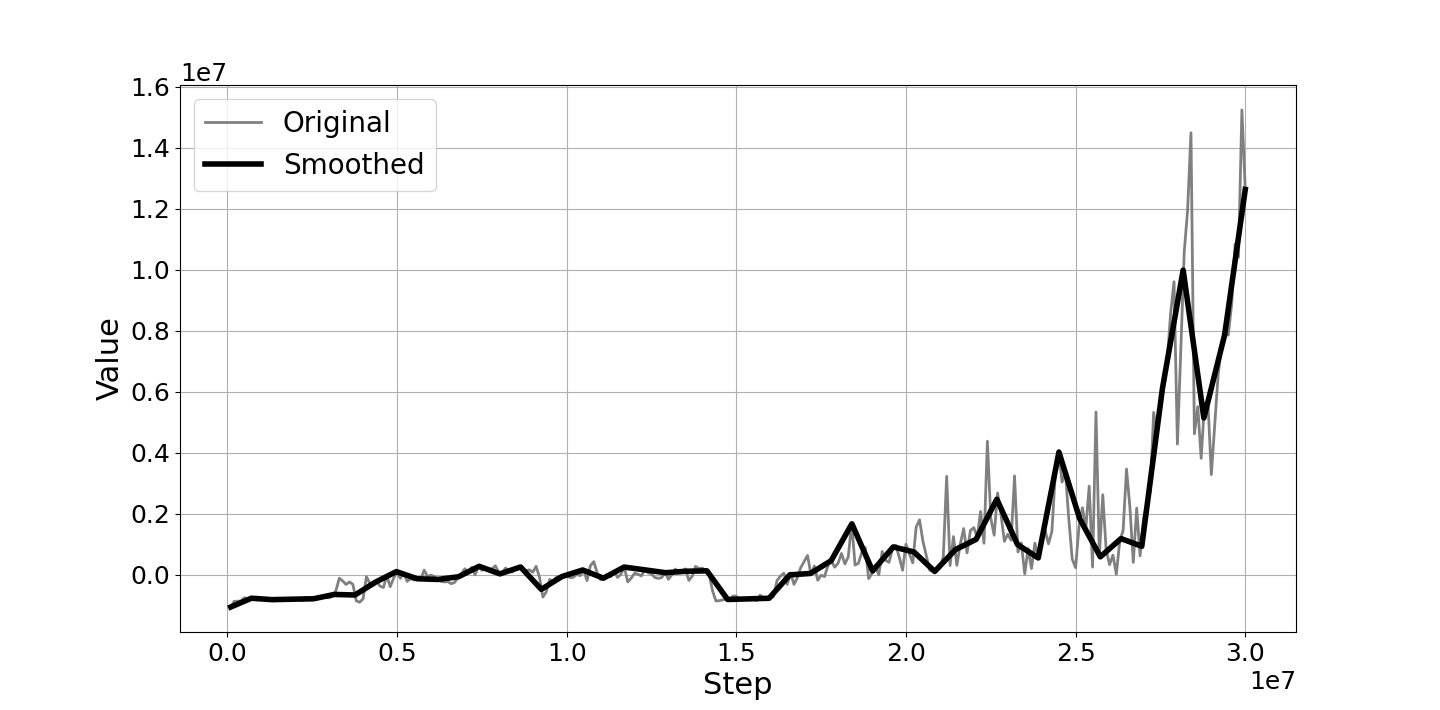
\includegraphics[width=1.0\linewidth]{figures/hardware_result/acrobot_learning_curve_real_world.png}
    \caption{Training curve of best result in acrobot setup}
    \label{fig:acrobot_training_curve}
\end{figure}

The behavior of this agent during ideal validation is shown in Figure \ref{fig:acrobot_ideal}. The swing-up is performed by the SAC controller within 2 seconds. After the LQR controller takes over, the system maintains stability around the highest position for a prolonged period. The ideal validation is considered successful.

\begin{figure}[H]
    \centering
    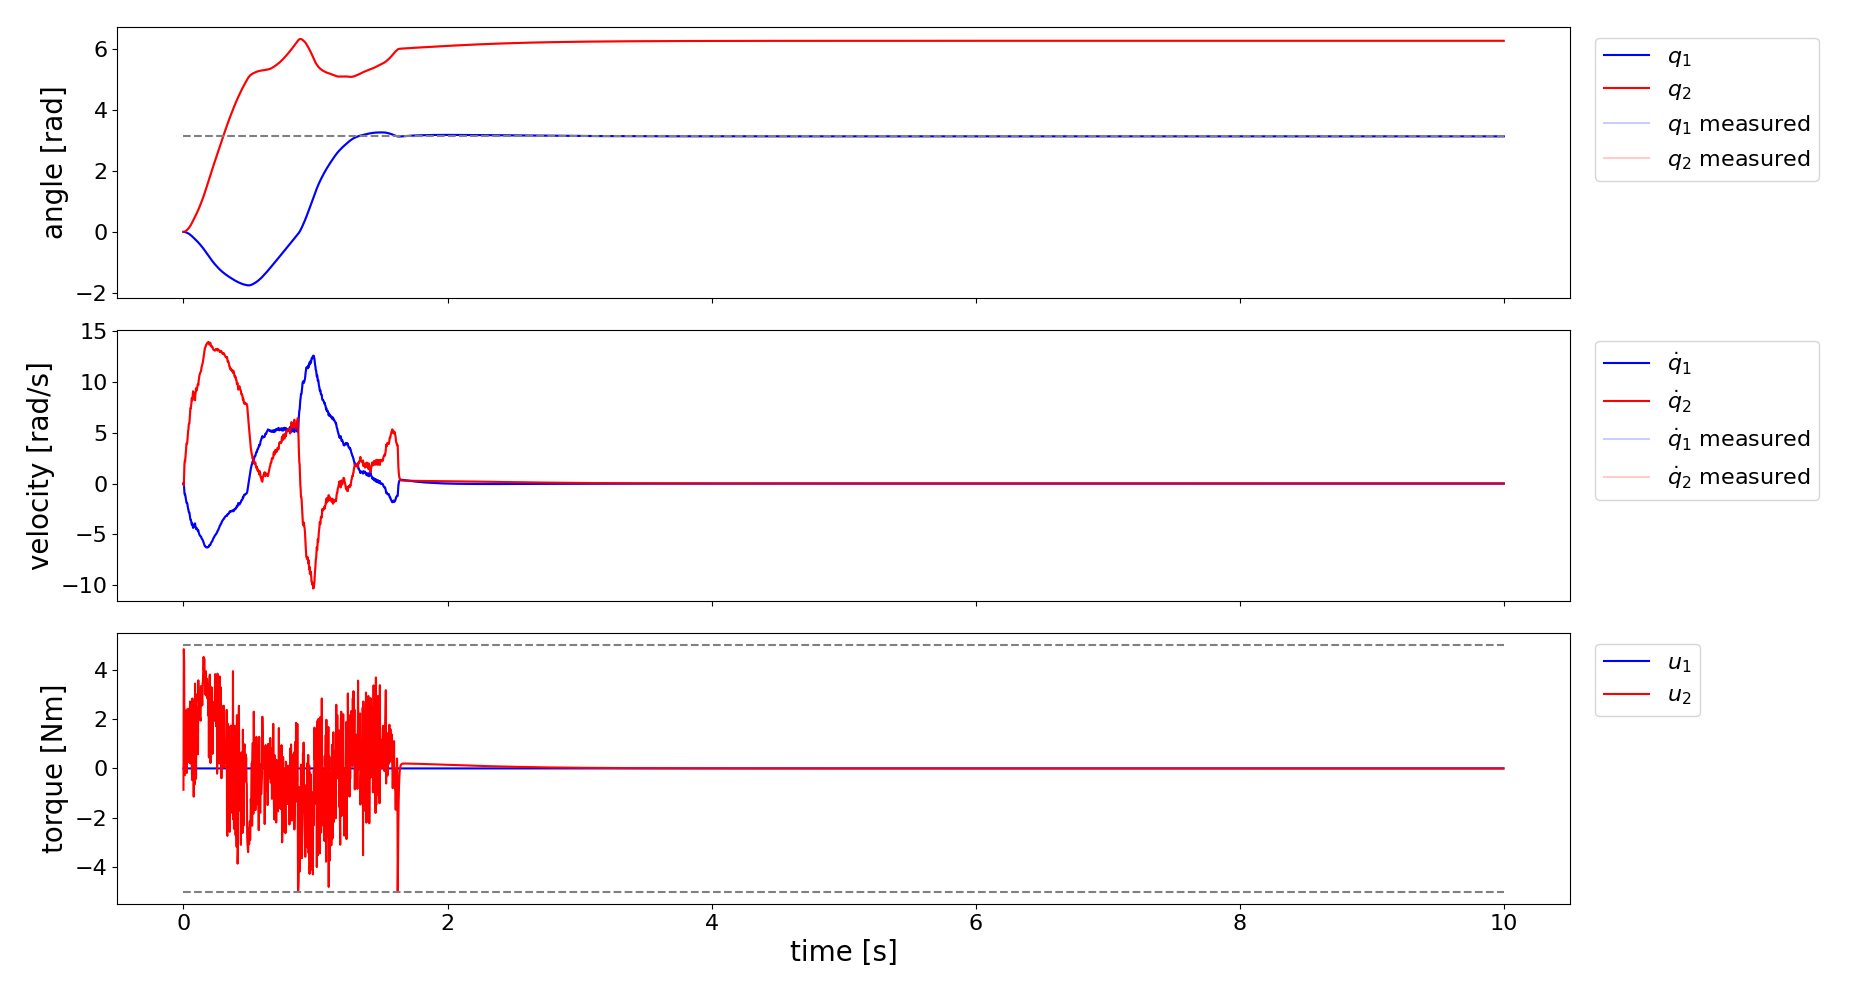
\includegraphics[width=0.95\linewidth]{figures/hardware_result/acrobot_ideal_simulation_designC.1.png}
    \caption{Acrobot result in ideal environment}
    \label{fig:acrobot_ideal}
\end{figure}

The agent operates successfully within a noisy simulation after ideal validation, eliminating the need for further noisy training. The success rate is approximately 50\%. Figure \ref{fig:acrobot_noisy} shows one of the successful tests.

In successful trials, the swing-up phase conducted by the SAC controller concludes within 2 seconds. Although the torque applied in ideal environment tests is already quite noisy, the torque in a noisy environment exhibits even greater fluctuations. Once the LQR controller takes effect, the system stabilizes around the goal state until the experiment concludes. In unsuccessful trials, the inability to switch to the LQR controller is the primary issue. But the agent has high recovery ability, the system sometimes misses the first transition oppotunity and making several rotations before it finds itself reaching a point for LQR controller to take over.

\begin{figure}[H]
    \centering
    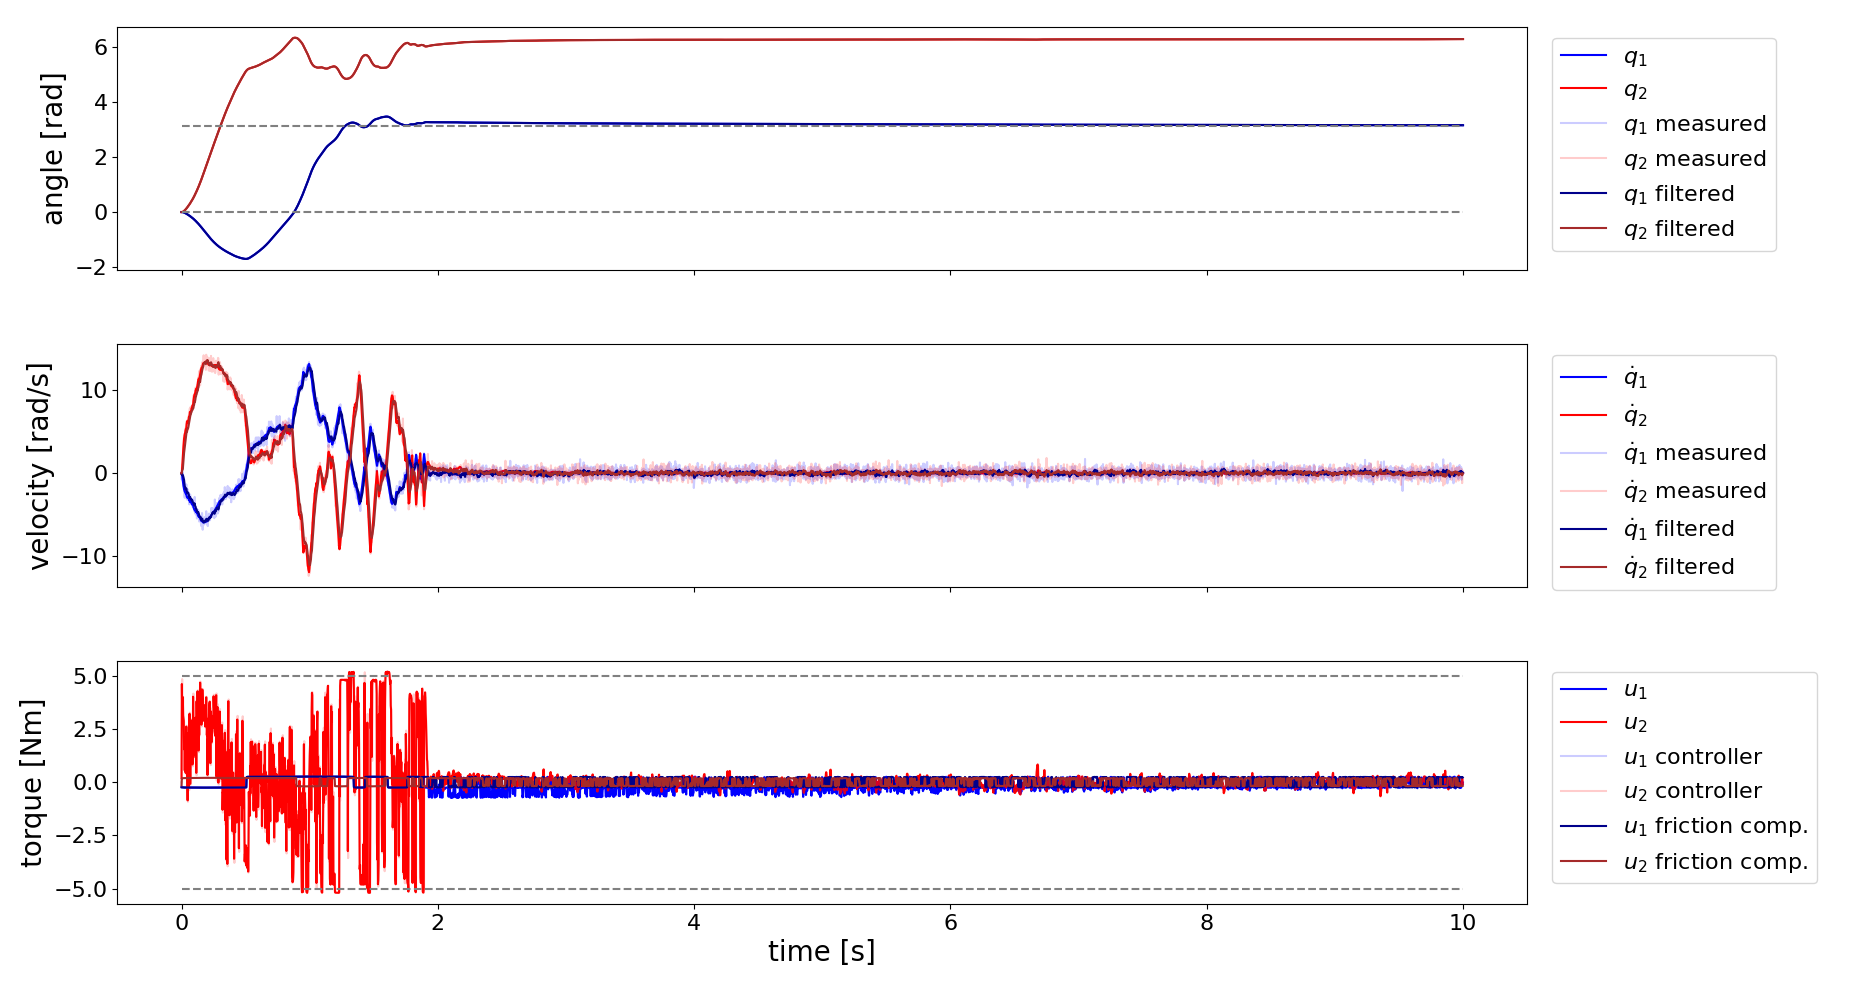
\includegraphics[width=1.0\linewidth]{figures/hardware_result/acrobot_noisy_simulation_designC.1.png}
    \caption{Acrobot result in noisy environment}
    \label{fig:acrobot_noisy}
\end{figure}

Due to the agent's violation of the \(2\pi\) position limit, it has been deemed unsuitable for real-world tests. Consequently, no additional results from real-world tests in the acrobot setup are presented.

\cleardoublepage
